\pgfsetplotmarksize{0pt}
\begin{figure}
 \centering
 \caption{\label{fl_conv6}UflLib/Euclid/1011EuclS.txt},
 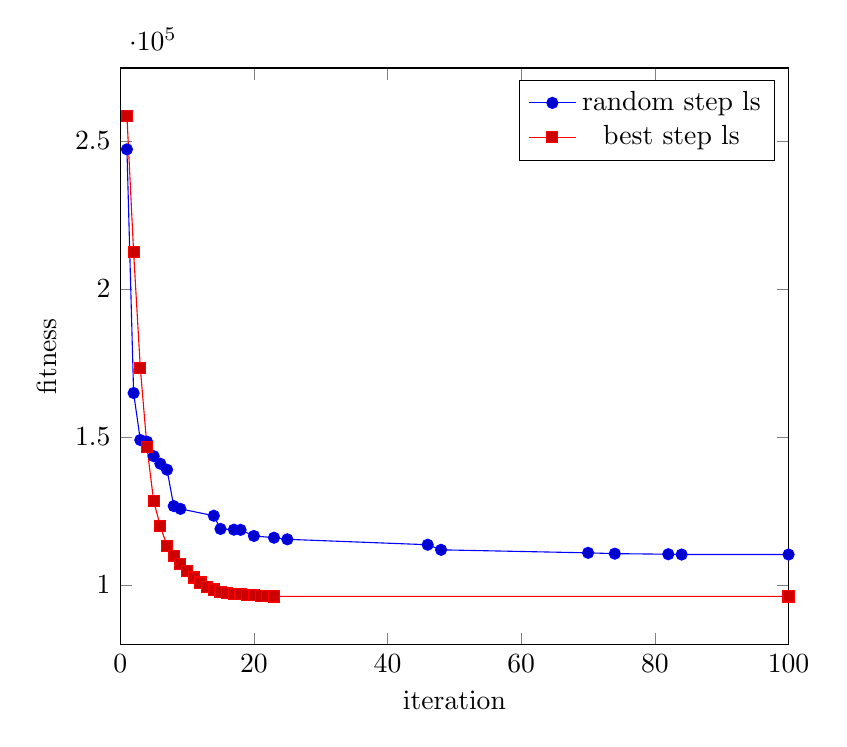
\begin{tikzpicture}
 \begin{axis}[
   width=0.7\textwidth,
   scale only axis,
   xlabel=iteration,
   ylabel=fitness,
   xmin=0,xmax=100,
   domain=0:100]
   \addplot coordinates {
     (0,inf)
     (1,247173)
     (2,164855)
     (3,148983)
     (4,148438)
     (5,143524)
     (6,140956)
     (7,138947)
     (8,126665)
     (9,125722)
     (14,123396)
     (15,118937)
     (17,118697)
     (18,118633)
     (20,116575)
     (23,115980)
     (25,115436)
     (46,113604)
     (48,111881)
     (70,110862)
     (74,110592)
     (82,110399)
     (84,110288)
     (100,110288)
   };
   \addlegendentry{random step ls}
   \addplot coordinates {
     (0,inf)
     (1,258418)
     (2,212384)
     (3,173393)
     (4,146526)
     (5,128358)
     (6,119830)
     (7,113211)
     (8,109737)
     (9,107133)
     (10,104709)
     (11,102534)
     (12,100826)
     (13,99429)
     (14,98453)
     (15,97721)
     (16,97269)
     (17,96972)
     (18,96841)
     (19,96724)
     (20,96670)
     (21,96416)
     (22,96355)
     (23,96135)
     (100,96135)
   };
   \addlegendentry{best step ls}
 \end{axis}
 \end{tikzpicture}
\end{figure}
